% try to get hyper links working

\title{	
	\normalfont\normalsize
	\textsc{University of Toronto}\\ % Your university, school and/or department name(s)
	\vspace{25pt} % Whitespace
	\rule{\linewidth}{0.5pt}\\ % Thin top horizontal rule
	\vspace{20pt} % Whitespace
	{\huge Student Engineering Handbook}\\ % The assignment title
	\vspace{12pt} % Whitespace
	\rule{\linewidth}{2pt}\\ % Thick bottom horizontal rule
	\vspace{12pt} % Whitespace
}
\author{\LARGE Hannah Brooks} % Your name
\date{\normalsize\today} % Today's date (\today) or a custom date

\documentclass[paper=a4, fontsize=11pt]{article} % A4 paper and 11pt font size
\usepackage[a4paper, total={6.5in, 9in}]{geometry}
\usepackage{graphicx}
\usepackage{setspace}
\usepackage{hyperref}
\usepackage{float}
\usepackage{enumitem}
\usepackage{lipsum}
\usepackage{sectsty}

\newcommand{\raisetarget}[2]% #1 = label, #2 = contents
{\bgroup
  \sbox0{#2}%
  \raisebox{\ht0}{\hypertarget{#1}{}}\usebox0%
\egroup}

\begin{document}
\maketitle
\newpage
\tableofcontents
\newpage


\section{Identity}
I am many things. I could go on and on about my hobbies and favourite pass times. I could tell you all about what sets me apart from Jane Doe: I play hockey. I love cooking. I'm from Ottawa. I volunteer in my free time. But why do these things matter? They can tell you about what makes me different as an engineer. They tell you what I bring to the table to create, improve or adapt a design solution and do it uniquely.

People have asked me before, ``Why did you decide to go into engineering?" My answer is always along the lines of, ``I want to be able to solve problems." In today's world, so much changes everyday: we witness countless stories of engineers changing people's lives, communities, and the world with their inventions.  So now, one year into my engineering degree, when people ask me why I chose engineering I say it’s because I could not imagine myself feeling more rewarded in any other discipline.

\begin{figure}[H]
    \centering
    \includegraphics[width=0.7\linewidth]{hockey.jpg}
    \caption{Picture from the Mice vs. Skule game!}
\end{figure}

This study of implementing simple designs with accessibility, sustainability, and efficiency in mind is simply the most rewarding experience I could be a part of.  Being a part of a team that allows me to identify a problem, create and deliver interventions as well as address the barriers of access to these creations, brings me a profound sense of purpose and meaning. Engineering for me is the study of how solutions can be designed simply and to work as efficiently as possible.

Over the past eight months, I have witnessed how each aspect of engineering comes together; from the heavy math to creative design, it truly became one in my eyes. This year I had the opportunity to be a part of numerous projects.  These included: creating a bridge design proposal in Toronto, creating a catapult which taught me the importance of the meticulous work required for a design before the physical creation, as well as propose unique designs for two communities based on their individual objectives \cite{objectives} and requirements \cite{requirements}. With each experience, I discovered the importance of using specific tools and techniques over others as well as learning how I identify as a novice engineer.

\begin{figure}[H]
    \centering
    \includegraphics[width=0.7\linewidth]{purple.jpg}
\end{figure}

One of the things I pride myself on is my communication skills, I love turning strangers into friends, learning about people's stories, and being social with those around me. My love for communication, learning people's stories, and connecting with those around me is how I've come to place such a high priority on stakeholder satisfaction. Validation \cite{validation} is a crucial component to successful solutions, this is attainable from understanding your stakeholders' needs as well as aligning them with your values. Second, I have had the opportunity to interact with many stakeholders in countless situations from my volunteer work at nursing homes to local community centers, this has helped equip me with skills for different positions.

\begin{figure}[H]
    \centering
    
\includegraphics[width=0.8\linewidth]{headshop.jpg}
\end{figure}

In my free time, I am a member of the university's solar car racing team, where I work as a part of the IT team; keeping the workstations available and ready for use, as well as running vulnerability tests and organize software are some of the many tasks I’m happy to do.  My dedication to the team has shown my readiness and flexibility in solving any variety of problems that may arise.  An example I can recall was when I had to create more user accounts for a specific node, it was a lengthy and tiresome process, however, after analyzing the problem from different points of view and brainstorming, I converged to the idea of automating the process using Ansible, an automation engine.  This way of thinking outside the box has shown me how to improve every design I make and ensure that the solution presented is as efficient as possible. 

\begin{figure}[H]
    \centering
    \includegraphics[width=0.5\linewidth]{toaster.jpeg}
    \caption{Knoll set up of our toaster tear-down.}
\end{figure}

Something that has always caused confusion for me was when people created unnecessarily complicated solutions.  The majority of the time there is no need for an elaborate setup and costly innovation.  With the wise words of Professor Collins playing in my ear, ``Keep It Simple Stupid," is a phrase that has served me well in my work, and will hopefully have a positive influence on any future project I may work on.  

\begin{figure}[H]
    \centering
    \includegraphics[width=0.5\linewidth]{jump.jpg}
\end{figure}

In my intense studies of physics, math, and chemistry, I have not only learned, but indeed bore witness to the value of meticulous work, it is something I will carry with me when I think of future designs.  The cohesive marriage of efficiency, simplicity, and dedication that engineering has shown me has led me to models that are unique and strong enough to face any obstacle head-on.
 
 
\section{Products of Personal Design}
    \subsection{CIV102 Bridge Design}
        \begin{figure}[H]
            \centering
            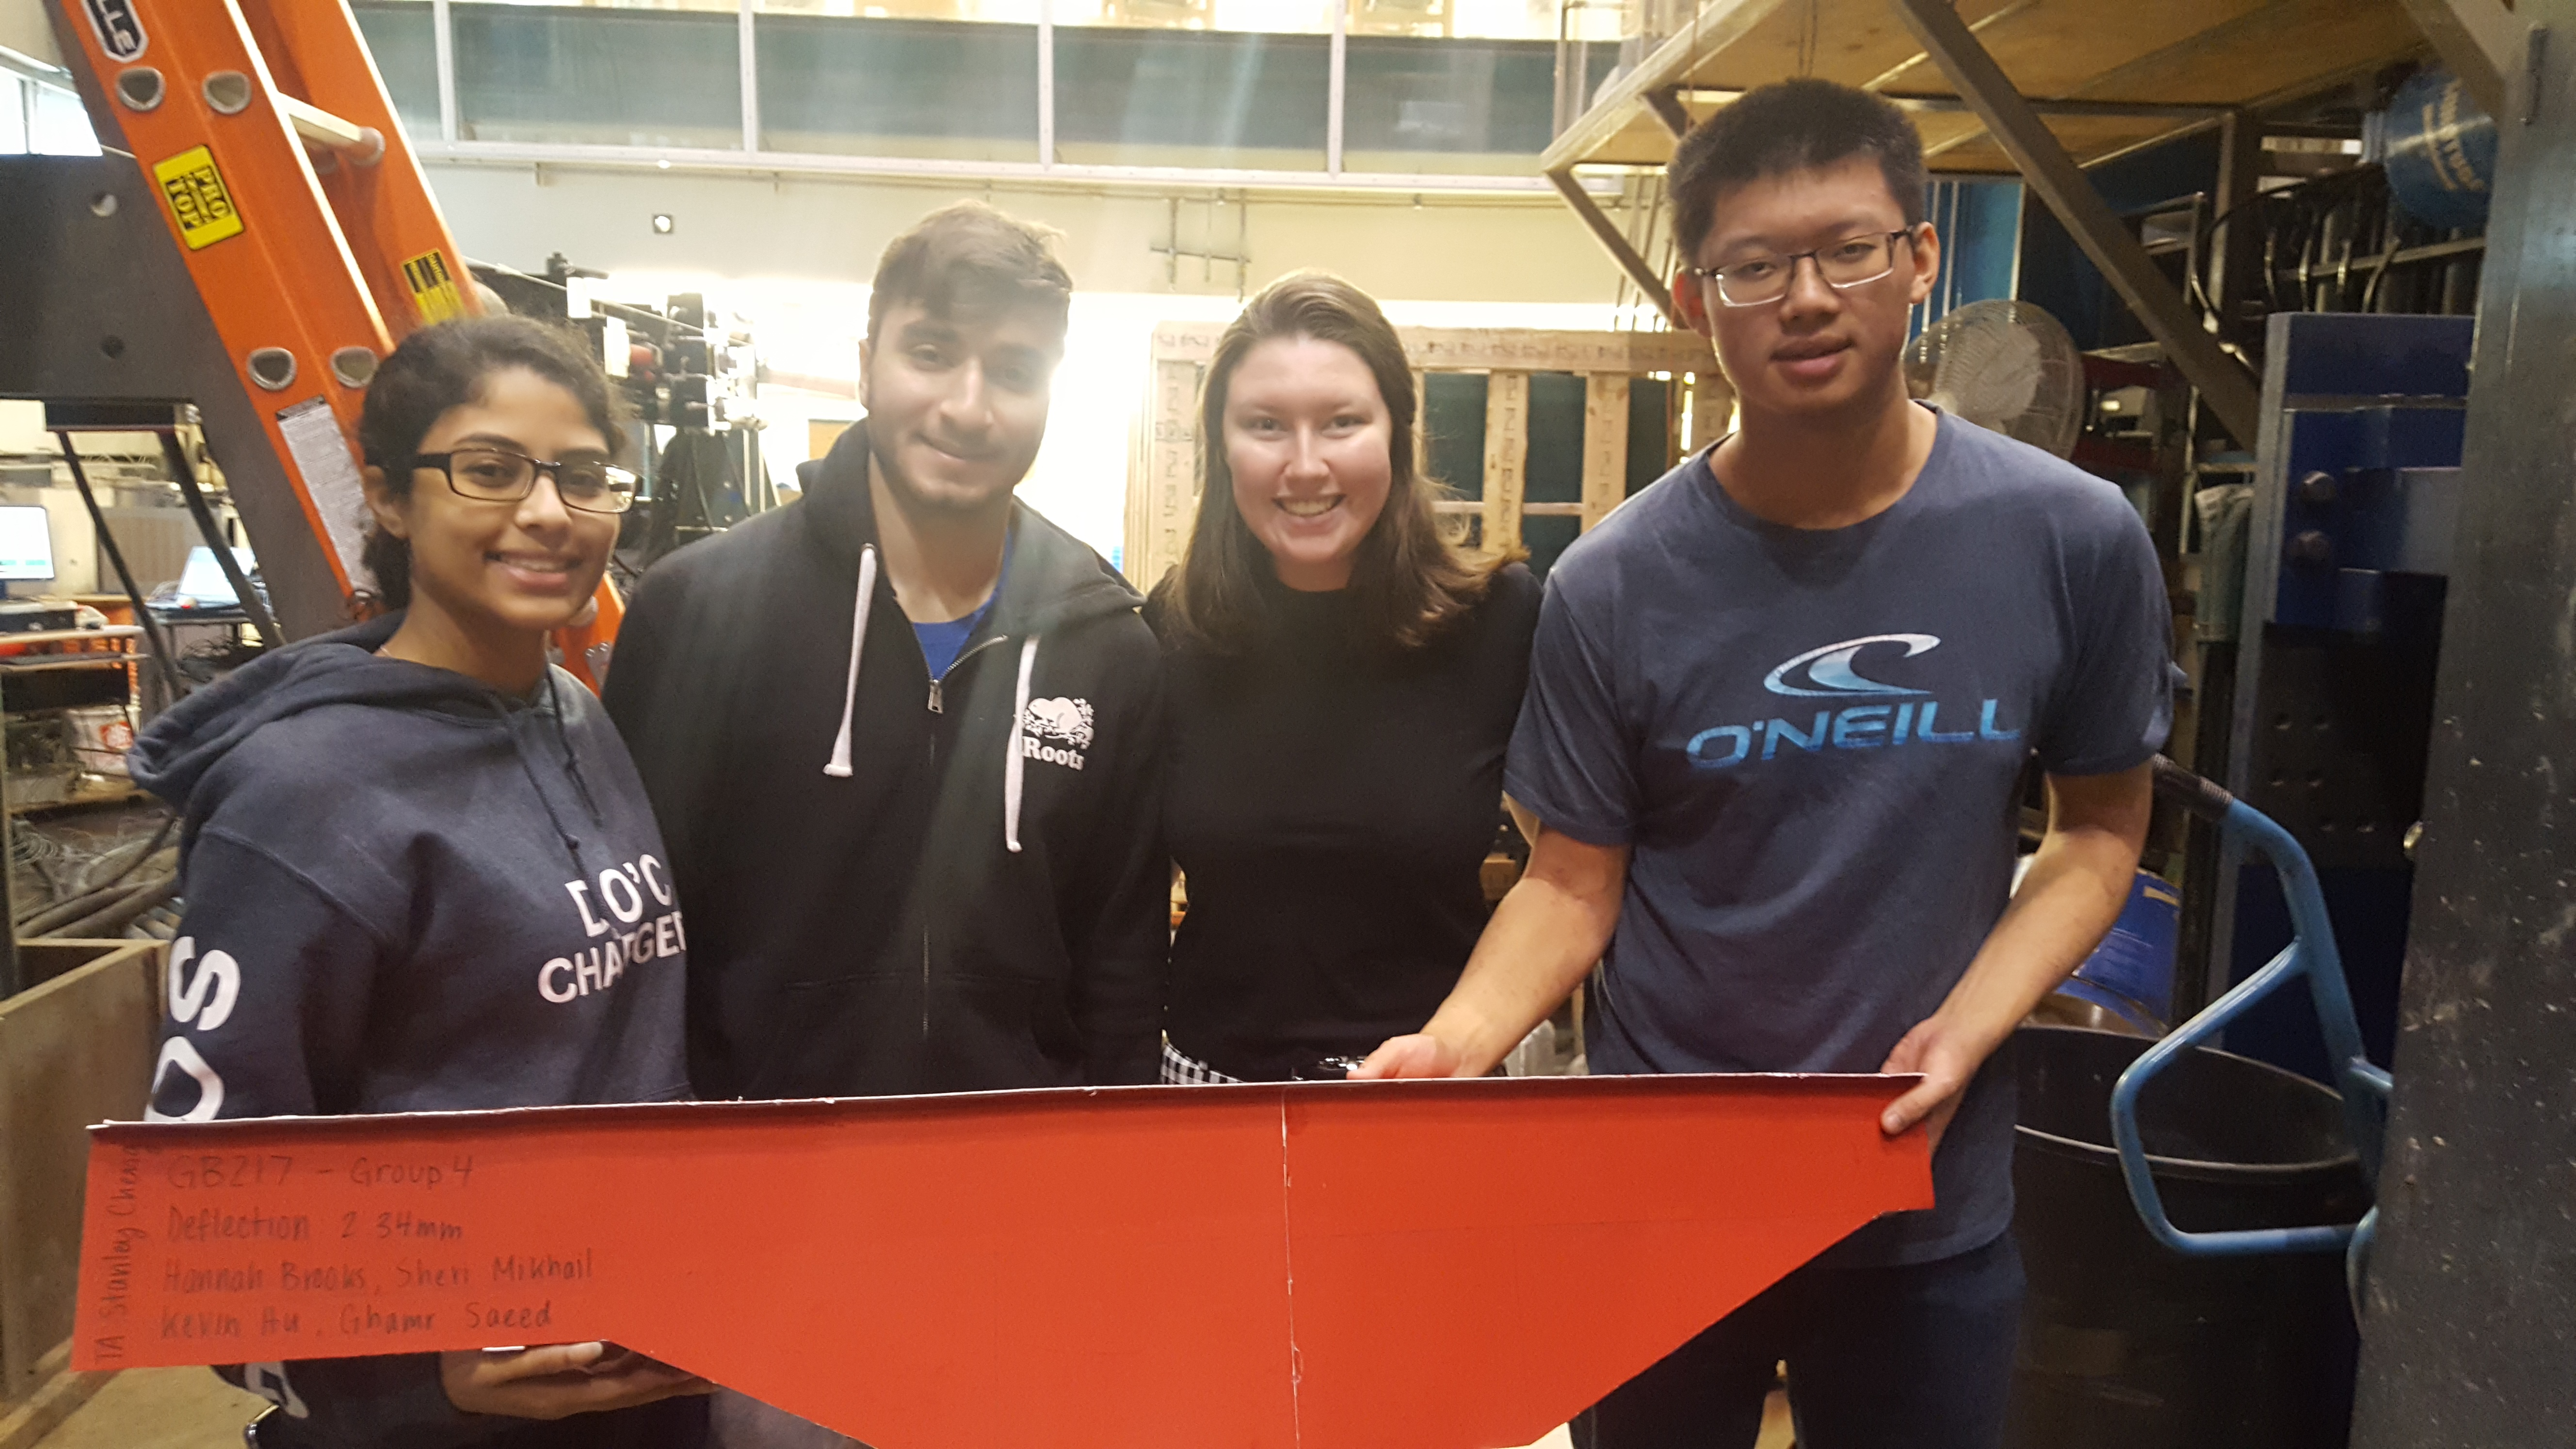
\includegraphics[width=0.6\linewidth]{bridgegroup.jpg}
            \caption{Part 2 - Our team picture with the final bridge.}
        \end{figure}
        \paragraph{Overview}
        The Bridge Design Project is a CIV102 project that has been going on for years. It has two parts: the ``Truss Bridge Design Request for Proposal" and the ``Bridge Design and Construction Competition". The first part I was in a group with Elif and Jondy. We visited the Glen Road Pedestrian Bridge and created a Personal Design Decision for the bridge with regards to new lighting across the bridge. After that, we designed a truss bridge to replace the existing bridge, drew both bridges and did all the necessary calculations.
        \newline
        The second part of the project is where you construct a bridge out of Matboard. In this group I was with Sheri, Ghamr and Kevin. We had to construct a bridge to span 1060mm, hold a train set weighing 400N and finally be tested to failure by the Baldwin. Our bridge safely passed the train test and failed at about 383N under the Baldwin. This was partially due to poor construction and partially due to poor design. If you wish to see a video of our bridge, you can find it \href{https://youtu.be/qZL1Y6M1oTY}{\textbf{here}}.
        \begin{figure}[H]
            \centering
            \includegraphics[width=0.7\linewidth]{drawing.jpg}
            \caption{Part 1 - The bridge drawings.}
        \end{figure}
        \paragraph{Design Process}
        The design process for part 1 was pretty standard. In terms of the PDD, we browsed catalogues and used selection design \cite{typesofdesign} to chose a light fixtures. There is a very limited number of street-grade lighting so the research was fast. For the bridge design, the dimensions were very specific and thus the constraints \cite{constraint} left little room for creativity. A deck-truss was chosen as a means of expressing the little creativity that we had and the calculations were performed from there. There was not much design that went into this section.
        
        For part two, we first began by looking at the class of 2011 for inspiration. The video can be found \href{https://www.youtube.com/watch?v=_g5RdcZs7tY}{\textbf{here}}. This team won second place during their year. Based on both their design design and other reference designs and various discussions it became obvious that webs with uniform height would not fair very well because of the varying moments. Thus, we decided that our bridge must have a varying height. No tools were used for this part of the process. We then made a python program that was supposed to calculate the moment and the varying height at 100 mm intervals. The program did not work correctly, and we had no more time to fix it or come up with a new one. To solve this problem, we chose an arbitrary height of 100 mm and an angle of 25 degrees. From there we performed our calculations by hand. The design of our bridge consisted of a pi beam with 17 diaphragms. 
        \begin{figure}[H]
            \centering
            \includegraphics[width=1\linewidth]{bridgecalcs.png}
            \caption{Part 2 - Code for inertia calculations of our bridge.}
        \end{figure}
        \paragraph{What I learned}
        In this experience, little to no engineering tools or techniques were used. This meant that we did not iterate over any prototypes to see which performed best, we did not weight different options against any other and we did not even determine that the design that we went with was the best. This effectively led to the downfall of our bridge. Due to ill-planning, we did not use our Matboard as efficiently as possible and did not use the correct proportions to optimize the moments of inertia. For next time I would plan out different designs and see how each prototype behaves in a simulated environment before converging to one final design.
        \begin{figure}[H]
            \centering
            \includegraphics[width=0.6\linewidth]{bridge1.jpg}
            \caption{Part 2 - Ghamr and Kevin building the bridge.}
        \end{figure}

    
    \subsection{Design for Commuters}
        \begin{figure}[H]
            \centering
            \includegraphics[width=0.6\linewidth]{praxis13.png}
            \caption{Mohammed, Richard and I at the end of a meeting.}
        \end{figure}
        \paragraph{Overview}
        It began with the Design Brief, followed by the Alpha Release and Design Critique and finally Design Review. In Praxis I, we were given the task to write a design brief to create a physical product that improved the learning experience of Engineering Science undergraduate students that also supports commuting. My team chose sleep deprivation as an area to focus on. We had three candidate designs: the nap-pod, the pillow-hoodie and the sleeping bag backpack. We ended up going with the pillow-hoodie and completed our prototypes and testing using this concept. 
        \begin{figure}[H]
            \centering
            \includegraphics[width=0.6\linewidth]{praxis12.png}
            \caption{Mohammed, Paul and I during a meeting.}
        \end{figure}
        \paragraph{Design Process}
        My team used \hyperlink{listlink}{Listing} to first diverge and come up with sleep deprivation as an opportunity for design. We wrote our review and then moved onto concept creation. We diverged using \hyperlink{scamplink}{SCAMPER} and \hyperlink{bwlink}{BrainWriting} and quickly converged using \hyperlink{boardlink}{Borda Count}, \hyperlink{tourlink}{Tournament style comparison} and \hyperlink{pairlink}{Pairwise}. The latter pair helped us decide our most important metric; ability to fall asleep. We diverged again using \hyperlink{scamplink}{SCAMPER} and then finished over the diverge-converge cycles with a \hyperlink{pughlink}{Pugh Chart} and a \hyperlink{ratlink}{Ratings Matrix}. Finally, we presented our ideas at Critique and then completed the painful review to finish off the project.

    \subsection{RFP and Showcase}
        \paragraph{Overview}
        Showcase is similar to the CIV102 project, where this is a project that EngScis of years gone past have also completed. For us this year it was unique in that we had to collect field notes from around the GTA in order to find an opportunity. I collected mine at the ROM and it was a great experience. My team (R58) ended up going with Cassey's field notes, which was at the 700 David Hornell Air Cadet Squadron. She described the gap between the learning experienced by the level three cadets and the Air Cadet Program’s aerospace education goal, demonstrated by low grades on their aviation knowledge tests. We approached this opportunity with gammification. The concept is an educational video game, called Airborne Intern, designed to supplement the aerospace learning goals of the ACP. It is a role playing game that covers the level three aviation curriculum, through the use of non-player character interactions, and mini-games. 
       \begin{figure}[H]
            \centering
            \includegraphics[width=0.6\linewidth]{praxis23.jpg}
            \caption{Our team photo after our presentation at showcase :,).}
        \end{figure}
        \paragraph{Design Process}
        After our RFP went through, we began the designing. First we reframed our approach: we refined the curriculum, changed the game from a concept retention tool to a teaching tool, allowed wifi etc. After that we used \hyperlink{listlink}{Listing} and \hyperlink{bwlink}{BrainWriting} to find all possible games. Next, we converged using \hyperlink{sys1v2}{system 1} (past experiences) followed by the \hyperlink{treelink}{Tree Method} and \hyperlink{bordalink}{Borda Count} combined with a \hyperlink{pairlink}{Pairwise}. We diverged again using \hyperlink{scamplink}{SCAMPER} and then refined our options. Finally we converged using a \hyperlink{pughlink}{Pugh Chart} to arrive at three candidate desings: an RP video game, a cyclic board game and a classic card game. Prototypes were created for each and then a \hyperlink{ratlink}{Ratings Matrix} led us to our final concept of an RPG. We then researched best practices, more gammification and extensive teaching techniques that led us to Airborn Intern. 
        \begin{figure}[H]
            \centering
            \includegraphics[width=0.6\linewidth]{praxis22.png}
            \caption{Another late night video call with Louis, Cassey and Henry.}
        \end{figure}
        \begin{figure}[H]
            \centering
            \includegraphics[width=0.6\linewidth]{praxis21.jpg}
            \caption{Me at 0300 at Myhal trying to build a board game out of scrap paper for Beta Release in 12 hours.}
        \end{figure}

    \subsection{Launcher}
    \begin{figure}[H]
        \centering
        \includegraphics[width=0.53\linewidth]{launch3.jpg}
        \caption{Henry, Cassey and I with our finished launcher.}
    \end{figure}
    \paragraph{Overview}
    The Launcher activity, or ``Team Build Test" was one of my favourites of the year. We had to build a projectile launcher that would send ~something~ flying through the air to land on a tile in Myhal. You can see a video of the launcher in action \href{https://youtu.be/uYIhF1Nd8Os}{\textbf{here}}. Overall, I think we scored about 50\%. Our accuracy was horrible and the launches were unpredictable. But the activity was fun and a great way to apply new found construction skills. 
    \paragraph{Design Process}
    Our design was something similar to a crossbow. Why, you ask? Well, because crossbows are cool; it's as simple as that. We had no process of legitimate design behind our creation. I recall us doing minor calculations but that sheet is now somewhere in the Light Fabrication Facility never to be seen again. We went off of intuition that a 45 degree angle would be optimal for projection. We tried to calculate the best angle, but without reference for the actual speed that it would be launched at, the task was lost on us. Thus we pressed on with our endeavour to build this thing. We hit Home Hardware, grabbed some plywood and came back to the LFF to build it. Louis did most of building. We tested our two different kinds of bungee cords and determined by a simple pull test that the black ones worked best. Finally, it came time to decide on the projectile. We had the issue that things would roll whenever they were shot. Thus we decided to use Play-Doh in order for it to stay in one place. This was also the only material that we could get our hands on in the short time period. There was no design thought behind this either. We tested in the corridors of Myhal (50 trials) and marked the ideal pull-back length. When we were pleased with the accuracy, we all went to get bubble tea. It was great team bonding (the tea and the projectile).
    \paragraph{What I learned}
    What I think the most important lesson was for this project is to have reasoning behind every decision made. Despite this being the grounds for much of Praxis, it escaped us on this occasion and we ended up with a cross bow/launcher that performed well below the standard. 
    \begin{figure}[H]
        \centering
        \includegraphics[width=0.5\linewidth]{launch2.jpg}
        \caption{Our team's launcher and I.}
    \end{figure}

\section{Visualization of the Design Process}
    \begin{figure}[H]
        \centering
        \includegraphics[scale=0.95]{flowchart.png}
    \end{figure}
    \paragraph{Description}
    My Personal Engineering Design Process takes inspiration from the French Design Process \cite{french}. The general process follows the method of first finding a valid opportunity, then working through three iterative processes, with constant feedback, until the proposed concept is validated.
    
    \paragraph{Processes}
    Adapted from the paper by Cross \cite{cross}, ``Conceptual Design and Embodiment Design".
        \begin{enumerate}
            \item \textbf{Problem Analysis}
             Leads to a problem statement which includes the Engineering Requirements Model \cite{erm}.
            \item \textbf{Conceptual Design}
             Created various solution in the form of concepts, using the original problem statement. In this stage is where reframing often occurs as lack of conceptual design can occur.
            \item \textbf{Embodiment Design}
             Convergence towards one solution occurs using multiple techniques.
        \end{enumerate}
    \paragraph{Connection to my Identity}
    This process allows me to approach each problem with a solution-oriented mindset instead of a problem-oriented mindset through the feedback loop and continuation of each process. Stakeholders are also constantly being taken into account with their input being taken in each iteration. Further, a design process that forces me to take part in idea-generation activities and assess my designs at each stage is key to creating an efficient design. Instead of going with ç takes over and leaves you with a Superior final concept.

\section{Tools, Models, Frameworks}
    \subsection{Framing}
        \subsubsection{Engineering Design Model}
            \begin{figure}[H]
                \centering
	            \includegraphics[width=0.6\linewidth]{designmodel.png}
	            \caption{The Engineering Design Model.}
            \end{figure}
            \paragraph{How I have used it in the past}
            \cite{edm} This model is the basis for all of the engineering practices that I have done. In order to begin a model, we must look at the world how it is, and envision how it could be improved. All factors of design play into this. In order to frame a situation, we must see how the world behaves and acts currently, and then dream how it could be. I used this technique primarily in my field note collection assignment and in both Praxis courses.
            \paragraph{Why}
            An opportunity is found in seeing how the world can be adapted, improved or created differently.
            \paragraph{When it's useless}
            This technique is never useless and is constantly used. Everywhere you look there is an opportunity for design. That couch over there, the lighting fixtures or that park bench can always become better.
            \paragraph{Future use}
            I have used this technique for the past eight months, I am currently using it, and hope that I will  never stop using it.
            \begin{figure}[H]
                \centering
	            \includegraphics[width=0.6\linewidth]{rom.jpeg}
	            \caption{Exploring accessibility at the ROM.}
            \end{figure}
        \subsubsection{Stakeholder Input}
            \begin{figure}[H]
                \centering
	            \includegraphics[width=0.6\linewidth]{cadets.jpg}
	            \caption{Cassey, Henry, Louis and I with the level three cadets.}
            \end{figure}
            \paragraph{How I have used it in the past} As mentioned earlier in the identity section, I hold stakeholder satisfaction as my top priority. In every design decision, my team and I tried to ensure that stakeholders were consulted in every step during the design process.
            \paragraph{Why} Without stakeholder approval, it is hard to claim that your design is successful. Further, as a part of my values, validation \cite{validation} is the most part of my process. 
            \paragraph{When it's useless} If you do not require stakeholder approval, or you are not designing with stakeholders in mind, then this aspect of framing will me meaningless to you. For example, the launcher project had our team as stakeholders, and no one else. This lead to minimal stakeholder interaction. 
            \paragraph{Future use} I hope to interact with many stakeholders in the future and take this mindset with me to every design scenario. 
    \subsection{Divergence}
        \raisetarget{bwlink}{}
        \subsubsection{BrainWriting}
            \begin{figure}[H]
                \centering
	            \includegraphics[width=0.8\linewidth]{brain1.jpg}
	            \caption{An example of BrainWriting to come up with mini-games for Praxis II.}
            \end{figure}
            \paragraph{How I have used it in the past}
            \cite{brainw} I have used BrainWriting not only in almost every design product in my first-year, but in every project I've ever done. BrainWriting is essentially the default brainstorming technique. You are writing out everything that comes to mind and it has helped my team dig our feet in to start a diverging process. 
            \paragraph{Why}
            You use BrainWriting to individually come up with ideas and the joint them later with your team. It helps to come up with many different ideas and get unique ideas that are completely crazy.
            \paragraph{When it's useless}
            This technique is useless if you have already done multiple rounds of it and you are creatively burnt out. It also doesn't help if you already have done good brainstorming and you're just looking to elaborate. It would be better to use a more refined tool in this case.
            \paragraph{Future use}
            I believe that I will use this tool whenever I need ideas. It's very easy to just jot down whatever you're thinking and just go where your mind takes you.
            \begin{figure}[H]
                \centering
	            \includegraphics[width=0.8\linewidth]{brain2.jpg}
	            \caption{An example of BrainWriting to come up with mini-games for Praxis II.}
            \end{figure}
            
        \raisetarget{listlink}{}    
        \subsubsection{Listing}
            \begin{figure}[H]
                \centering
	            \includegraphics[width=0.6\linewidth]{list2.jpg}
	            \caption{An example of using Listing to brainstorm for showcase.}
            \end{figure}
            \paragraph{How I have used it in the past}
            \cite{listing} Listing can be seen as a combination of \hyperlink{bwlink}{BrainWriting} and a mind map. It helps to organize the ideas that you are writing down into ways that you see fit. It isn't as wild as a mind map, but it still gives you the freedom to write everything that you need. I use it frequently in my day-to-day whenever I need to organize my thoughts but I also used it in Praxis I and Praxis II.
            \paragraph{Why}
            You can use the Listing technique of brainstorming to organize your ideas in an analogue way in order to keep your thoughts in order. It is best used for calm brainstorming session and for early on brainstorming. However it can also be integrated into other brainstorming techniques to get the most out of your session.
            \paragraph{When it's useless}
            Listing is not useless very often. In fact, it is used almost everywhere and is seen in many design activities. It is only useless if the categories of the lists are ill-chosen and confuse the team.

            \paragraph{Future use}
            Listing is a tool I use often and will hopefully continue using. It could also be applied to many different aspects of life: work, hobbies, lifestyle choices, closet organization etc. and I look forward to seeing where Listing takes me.
            \begin{figure}[H]
                \centering
	            \includegraphics[width=0.8\linewidth]{list.png}
	            \caption{An example of using Listing to brainstorm for problems for commuters in EngSi.}
            \end{figure}
        \raisetarget{treelink}{}
        \subsubsection{Tree Method}
            \paragraph{How I have used it in the past}
                    \cite{tree} The tree was a very specific type of brainstorming and idea generation for us. It was the first time that I had ever used it. There were many types of video games that needed to be organized and the easiest way to do this was to categorize. We drew on our computer science knowledge and created a general tree to store our data items.
                    \paragraph{Why} You use this tool in order to visualize many ideas that are all similar and linked together in some way. It allows you to understand the connection between items and distinguish between their features.
                    \paragraph{When it's useless} If you have a very limited amount of concepts that are randomly selected, this tool will not be very useful. If your concepts are all going in different directions, the ability to visualize the links between them will not benefit your divergence process. 
                    \paragraph{Future Use} I would hope to use this to organize everyday tasks, use it to weigh options (if a binary tree was used) and to use it for creative divergence on one concept. 
                    \begin{figure}[H]
                        \centering
	                    \includegraphics[width=0.6\linewidth]{tree.jpg}
	                    \caption{Louis and Henry talking about our tree brainstorm.}
                    \end{figure}
        \raisetarget{scamplink}{}
        \subsubsection{SCAMPER}
            \paragraph{How I have used it in the past}
             \cite{scamp} I have used SCAMPER in almost every divergence I have done. I believe that this is because it is a go-to example for a brainstorming tool. I have never really liked it because it is too long to be useful. Usually my team gives up after ``A''. I used it prominently in Praxis I, the launcher and Praxis II. 
            \paragraph{Why}
            SCAMPER helps to get improve or build on your current concepts. It will help you create minor differences in the items already chosen to go forward with. 
            \begin{figure}[H]
                \centering
	            \includegraphics[width=0.8\linewidth]{scamper2.jpg}
	            \caption{Cassey and I working on Praxis II project.}
            \end{figure}
            \paragraph{When it's useful/useless} It is extremely useful to generate iterations on current designs but not very useful to creating brand new ideas. Unless you complete multiple rounds of SCAMPER, a unique idea is unlikely to present itself. 
            \paragraph{Future Use} I wil hopefully not be using this tool again unless I am left without any other option. It was overused for me and did not live up to it's reputation. 

            \begin{figure}[H]
                \centering
	            \includegraphics[width=0.8\linewidth]{scamper1.png}
	            \caption{Stickie notes from SCAMPER in Praxis I.}
            \end{figure}
            
    \subsection{Convergence}
        \raisetarget{pughlink}{}
        \subsubsection{Pugh Chart}
            \begin{figure}[H]
                \centering
	            \includegraphics[width=1\linewidth]{firstpugh.png}
	            \caption{Pugh Chart in convergence cycle for Praxis I.}
            \end{figure}
            \paragraph{How I have used it in the past}
            \cite{pugh} The Pugh chart was the first convergence tool we were introduced to. It was the tool I used in my Personal Design Decision and it has been used heavily ever since. I really liked it when we were allowed to sum up the values as it gave a qualitative answer quickly and used \hyperlink{sys1v2}{system 1 thinking}. When we learned this was bad practice it disappointed me periodically, but ended up helping me make more educated decisions. This tool will be here to stay for me. 
            \paragraph{Why} Using a Pugh chart is an easy way to converge quickly and effectively using your metrics \cite{metrics}. It can also be used a way to judge how well your metrics \cite{metrics} gauge how well your concepts perform. 
            \paragraph{When it's useful/useless} It is useful to converge quickly and with low-fidelity prototypes. It is useless if your metrics \cite{metrics} do not distinguish well enough between the concepts. It also does not work as well when you have a small number of potential ideas. 
            \paragraph{Future Use} I will likely use this tool in all of my  future design endeavours. I have used it frequently and it has always helped to converge in every instance. 
            \begin{figure}[H]
                \centering
	            \includegraphics[width=1\linewidth]{spreadpugh.png}
	            \caption{Pugh Chart prepared for Showcase.}
            \end{figure}

            \begin{figure}[H]
                \centering
	            \includegraphics[width=1\linewidth]{pughbridge.png}
	            \caption{Pugh Chart to converge on the type of lighting for the bridge project in CIV102.}
            \end{figure}
        
        \raisetarget{ratlink}{}
        \subsubsection{Ratings Matrix}
            \begin{figure}[H]
                \centering
	            \includegraphics[width=0.6\linewidth]{bubblesratings.jpg}
	            \caption{Ratings matrix of types of games for Praxis II featuring Louis, Henry and I.}
            \end{figure}
            \begin{figure}[H]
                \centering
	            \includegraphics[width=1\linewidth]{spreadratings.png}
	            \caption{Ratings matrix of mini-games for Showcase.}
            \end{figure}
            \paragraph{How I have used it in the past}
            \cite{ratmatrix} I believe that this tool is arguably the most important one that we have been introduced to this year. It takes all aspects of the designs into consideration. I used it in Praxis I, Praxis II twice and it had proven very effective. 
            \paragraph{Why} The ratings matrix shows the value that each concept has and what its strengths are in different areas. It can compare it to others while also giving you the big picture of your candidate designs. 
            \paragraph{When it's useless}
            I really don't think that the ratings matrix is ever not useful, unless the chosen metrics \cite{metrics} do not align well for a matrix. 
            \paragraph{Future use}
            I hope to use the Ratings Matrix to help measure my candidate designs and compare them against each other for many designs to come. I could also apply it to my personal life with different tasks that I have to do.
            \begin{figure}[H]
                \centering
	            \includegraphics[width=0.6\linewidth]{firstratings.png}
	            \caption{Ratings Matrix for concepts in Praxis I.}
            \end{figure}
        \raisetarget{pairlink}{}
        \subsubsection{Pairwise Comparison}
            \begin{figure}[H]
                \centering
	            \includegraphics[width=0.6\linewidth]{pairwise.jpg}
	            \caption{Game convergence in early Praxis II project design.}
            \end{figure}
            \begin{figure}[H]
                \centering
	            \includegraphics[width=0.7\linewidth]{pairborda.png}
	            \caption{A mixture of Borda Count and Pairwise comparison for critical metric in Praxis I.}
            \end{figure}
            \paragraph{How I have used it in the past}
            \cite{pairwise} Similar to the \hyperlink{pughlink}{Pugh Chart} and \hyperlink{ratlink}{Ratings Matrix}, this was another tool that I used frequently. I used it for the first time in Praxis I in conjunction with a \hyperlink{bordalink}{Borda Count} when one of my group members suggested we try it. I also used it in Praxis II in the initial convergence steps.
            \paragraph{Why}
            Pairwise Comparison is an analytical way to evaluate your concepts and is used similarly to the \hyperlink{pughlink}{Pugh Chart} in order to converge quickly and efficiently. 
            \paragraph{When it's useless}
            Again, similar to \hyperlink{pughlink}{Pugh Chart} where if you have a small number of concepts it will become ineffective. However, if you also have a very large number of concepts, your matrix could become hard to interpret and confusing.
            \paragraph{Future use}
            I will hopefully use this in the future as a secondary design tool and use it to converge early and quickly.
        \raisetarget{tourlink}{}
        \subsubsection{Tournament Style Comparison}
            \paragraph{How I have used it in the past}
            \cite{tournament} I have only used Tournament style once in the past. I used it in Praxis I and it was effective but I think we only used it in order to say that we had used multiple convergence tools. I don't think it was actually helpful to our process, i.e. we could have converged without it and arrived at the same place. This tool is also good for sports fans.
            \paragraph{Why}
            You use it to determine theoretically which concept is the best. This runs along \hyperlink{sys1v2}{system 1 thinking} as there is no in depth reflection into what makes a concept superior to another.
            \paragraph{When it's useless}
            It is useless if you have very little concepts or if you need in-depth thinking to evaluate the candidacy of your designs.
            \paragraph{Future use}
            I don't think I will be using this tool very much in the future, unless I am making a bracket or if I have many concepts that I need a quick evaluation for.
            \begin{figure}[H]
                \centering
	            \includegraphics[width=0.8\linewidth]{tournament.png}
	            \caption{Tournament style convergence in Praxis I.}
            \end{figure}
        \raisetarget{bordalink}{}
        \subsubsection{Borda Count}
            \paragraph{How I have used it in the past}
            \cite{borda} I have used the Borda count multiple times. The teams that I have been on and I like it because it is democratic. Democracy is good. Everyone feels heard and it leads to a decision being made by the whole team and not just one person.
            \paragraph{Why}
            Use this tool if the other design techniques that you have used failed or if you need to eliminate a solution. It also helps if you are having a disagreement in the team to work things out.
            \paragraph{When it's useless}
            If you have too many topics and not enough votes to differentiate the topics enough to make a decision. It is also useless if you have communists or fascists on your team.
            \paragraph{Future use}
            I will hopefully use this in the future as a check-in tool with my team but also as a secondary convergence tool. It has been proven useful and thus it will hopefully serve me well again soon.
            \begin{figure}[H]
                \centering
	            \includegraphics[width=0.6\linewidth]{borda.png}
	            \caption{Borda Count in Praxis I for original ideas.}
            \end{figure}
    \subsection{Risk Management}
        \subsubsection{Gantt Chart}
            \paragraph{How I have used it in the past}
            \cite{gantt}Throughout the writing of our RFP, we used weekly schedules to keep ourselves on track. We did the same thing in in order to complete our project in showcase. They were not in the form of Gantt charts, but they were essentially were. I have included a photo of what they would have been if they were Gantt charts.
            \paragraph{Why}
            The weekly schedules/Gantt charts help keep teams on track to complete the task at hand and also helps prevent procrastination. Another benefit that they provide is that it can show which team member is in charge of which task to help keep the project organized.
            \paragraph{When it's useless}
            If your team is very laid-back and prefer working at their own pace without set deadlines, it is very easy to get frustrated with these tools. Further, if the set deadlines of each day are not met, it can become hard to keep up with the rest.
            \paragraph{Future use}
            I use an agenda everyday for everything I do and I love having a schedule for my projects. I will use hopefully use it both personally and in group projects int the future.
            \begin{figure}[H]
                \centering
	            \includegraphics[width=0.5\linewidth]{schedule.png}
	            \caption{Ratings Matrix of mini-games for Showcase.}
            \end{figure}
            \begin{figure}[H]
                \centering
	            \includegraphics[width=1\linewidth]{gantt.png}
	            \caption{What the schedule would look like as Gantt chart. Made 14/04/19.}
            \end{figure}
            \begin{figure}[H]
                \centering
	            \includegraphics[width=1\linewidth]{calendar.png}
	            \caption{My schedule for a week in February this semester.}
            \end{figure}
    \subsection{Miscellaneous}
        \subsubsection{AID Model}
            \paragraph{How I have used it in the past}
            \cite{aid} The Action, Impact, Desired outcome model is a feedback technique to provide effective construction on your team's performance and teammates behaviour. I have used it in Praxis I and Praxis II.
            \paragraph{Why}
            This model helped me get my point across in every Team Effectiveness Learning Survey that I have had to do. It outlines my thoughts and conveys them in a respectful, yet critical way.
            \paragraph{When it's useless}
            This model will be useless if your teammates are not up to recieving feedback or you have very simple thoughts that need to be brought up. It would be better to just express them.
            \paragraph{Future use}
            I hope to use this in future team evaluations as well as self-evaluations in the near future.
            \begin{figure}[H]
                \centering
	            \includegraphics[width=1\linewidth]{aid.png}
	            \caption{An example of the AID model in use.}
            \end{figure}
            
\begin{thebibliography}{50}
\bibitem{edm}
J. Foster and R. Irish, Class Lecture, Topic: ``Lecture 9", ESC101, Engineering Science, University of Toronto, Toronto, Ont., Sept., 2018

\bibitem{brainw}
M. Arivananthan and G. Salokhe, \textit{Brain Writing}. kstoolkit, July, 2018.
\\\texttt{http://www.kstoolkit.org/brain\_writing}
\begin{figure}[H]
    \centering
    \includegraphics[width=1\linewidth]{write.png}
\end{figure}

\bibitem{listing}
Mind Tools Content Team, \textit{Attribute Listing, Morphological Analysis and Matrix Analysis: Tools for Creating New Products and Services}. MindTools, 2019.\\\texttt{https://www.mindtools.com/pages/article/newCT\_03.htm}
\begin{figure}[H]
    \centering
    \includegraphics[width=1\linewidth]{listy.png}
\end{figure}


\bibitem{tree}
B. King, \textit{Brainstorming}. LinkedIn Slideshare, Jul. 2015. \\\texttt{https://www.slideshare.net/bking/brainstorming-50721336}
\begin{figure}[H]
    \centering
    \includegraphics[width=0.6\linewidth]{tree.png}
\end{figure}

\bibitem{scamp}
J. Foster and R. Irish, Class Lecture, Topic: ``Lecture 23", ESC101, Engineering Science, University of Toronto, Toronto, Ont., Nov., 2018

\bibitem{pugh}
J. Foster and R. Irish, Class Lecture, Topic: ``Lecture 9", ESC101, Engineering Science, University of Toronto, Toronto, Ont., Sept., 2018

\bibitem{ratmatrix}
J. Foster and R. Irish, Class Lecture, Topic: ``Lecture 32", ESC101, Engineering Science, University of Toronto, Toronto, Ont., Nov., 2018

\bibitem{pairwise}
J. Foster and R. Irish, Class Lecture, Topic: ``Lecture 17", ESC101, Engineering Science, University of Toronto, Toronto, Ont., Oct., 2018

\bibitem{tournament}
J. Foster and R. Irish, Class Lecture, Topic: ``Lecture 17", ESC101, Engineering Science, University of Toronto, Toronto, Ont., Oct., 2018

\bibitem{borda}
J. Foster and R. Irish, Class Lecture, Topic: ``Lecture 17", ESC101, Engineering Science, University of Toronto, Toronto, Ont., Oct., 2018

\bibitem{gantt}
J. Foster and R. Irish, Class Lecture, Topic: ``Lecture 14", ESC102, Engineering Science, University of Toronto, Toronto, Ont., Mar., 2019

\bibitem{french}
D. Wynn and P. Clarkson, \textit{Process models in design and development}. Research in Engineering Design, 2018.
originally from
\newline
M. J. French, \textit{Conceptual Design for Engineers}. Lancaster, UK: Springer, Berlin, Heidelberg, 1985. \\\texttt{https://link.springer.com/book/10.1007\%2F978-3-662-11364-6}
\begin{figure}[H]
    \centering
    \includegraphics[width=0.6\linewidth]{flow.png}
\end{figure}

\bibitem{cross}
N. Cross, \textit{Engineering Design Methods: Strategies for Product Design}. West Sussex, England: Wiley, 2000. \\\texttt{https://www.researchgate.net/publication/200026146\_Engineering\_Design\_Methods\_Strategie}
\\\texttt{s\_for\_Product\_Design}

\bibitem{civvid}
[username] Roxychic124, \textit{CIV102 Cardboard Bridge Testing - 1T5}. Youtube, Dec. 2011.
\\\texttt{https://www.youtube.com/watch?v=\_g5RdcZs7tY}

\bibitem{validation}
J. Foster and R. Irish, Class Lecture, Topic: ``Lecture 9", ESC101, Engineering Science, University of Toronto, Toronto, Ont., Sept., 2018

\bibitem{system1v2}
J. Foster and R. Irish, Class Lecture, Topic: ``Lecture 1", ESC101, Engineering Science, University of Toronto, Toronto, Ont., Sept., 2018

\bibitem{objectives}
J. Foster and R. Irish, Class Lecture, Topic: ``Lecture 6", ESC101, Engineering Science, University of Toronto, Toronto, Ont., Sept., 2018

\bibitem{requirements}
J. Foster and R. Irish, Class Lecture, Topic: ``Lecture 9", ESC101, Engineering Science, University of Toronto, Toronto, Ont., Sept., 2018

\bibitem{metrics}
J. Foster and R. Irish, Class Lecture, Topic: ``Lecture 9", ESC101, Engineering Science, University of Toronto, Toronto, Ont., Sept., 2018

\bibitem{typesofdesign}
J. Foster and R. Irish, Class Lecture, Topic: ``Lecture 4", ESC101, Engineering Science, University of Toronto, Toronto, Ont., Sept., 2018

\bibitem{constraint}
J. Foster and R. Irish, Class Lecture, Topic: ``Lecture 8", ESC101, Engineering Science, University of Toronto, Toronto, Ont., Sept., 2018

\bibitem{erm}
Engineering Science Wiki, 2019.
\\\texttt{https://wiki.engsci.utoronto.ca/index.php?search=requirements+model\&title=Special\%3ASea}
\\\texttt{rch\&go=Go}
\begin{figure}[H]
    \centering
    \includegraphics[width=0.6\linewidth]{erm.png}
\end{figure}

\bibitem{aid}
J. Foster and R. Irish, Class Lecture, Topic: ``Lecture 20", ESC101, Engineering Science, University of Toronto, Toronto, Ont., Nov., 2018

\end{thebibliography}

\end{document}
